\mainsection{\the\numexpr \thechapter + 1 \relax}{Fonctionnement d'un ordinateur}{27/09/1982}

%Théorie :
% Distinguer les types de mesure et leurs principaux ordres de grandeur.
%Comprendre les liens entre utilisateurs, périphériques, applications et systèmes d’exploitation.
%
%Pratique :
%Connaître le nom de plusieurs systèmes d’exploitation et les appareils sur lesquels ils sont installés.

\section{Système d'exploitation}
\begin{wrapfigure}[]{r}{0.3\textwidth}
	\centering
	\includegraphics[trim=0 0 0 0,width=0.25\textwidth]{Images/ordinateur/systemeexploitation}
	\caption{Les couches d'abstraction d'un ordinateur.}
\end{wrapfigure}
Vous souhaitez développer un nouveau programme pour smartphone qui va par exemple utiliser la caméra de votre appareil pour prendre des photos. Le problème c'est qu'il existe des centaines de modèles de caméras différent, donc il va vous falloir écrire des centaines de version différentes de votre programme qui chacune sera capable de gérer le bon modèle de caméra (communiquer, s'adapter à la résolution de l'image, etc.). Maintenant vous réalisez qu'il existe aussi des centaines de modèles d'écrans différent, rebelote, il faut de nouveau une centaine de version de votre programme qui devra gérer tous ces écrans et toutes les combinaisons possibles de modèles d'écrans et de caméras!\\

Pour faciliter les choses, on a inventé des programmes bien spécifique qui on pour but de créer un type d'interface (on parle aussi de couche d'abstraction) entre votre application et le matériel de votre ordinateur. Ce programme s'appelle un {\bf système d’exploitation}. Il va permettre à votre application de communiquer avec la caméra de manière générique, peu importe le modèle à partir du moment que la caméra fait des "trucs" de caméra (comme prendre des photos). C'est le système d'exploitation installé sur votre téléphone qui saura comment gérer un modèle spécifique de caméra. Dans ce contexte, il suffit de développer une seule application pour un système d'exploitation précis et l'application fonctionnera sur tous les téléphones qui ont ce système d'exploitation!
\begin{mydefinition}
	Le {\bf système d’exploitation} (noté SE ou OS, abréviation du terme anglais Operating System est un programme qui organise la liaison entre les ressources matérielles (mémoire, accès aux périphériques d'entrées/sorties), l'utilisateur et les applications (traitement de texte, jeu vidéo..). 
\end{mydefinition}	
On pourrait reprendre le même raisonnement que ci-dessus et déduire que pour chaque version d'un système d'exploitation il doit y avoir des centaines de versions différentes car, in fine, un système d'exploitation n'est rien d'autre qu'un programme. En fait, beaucoup de composant sont standardisés, c'est-à-dire qu'ils fonctionnent plus ou moins de la même manière ou avec un nombre restreints de variations. C'est le cas notamment des disques durs, mémoires RAM, souris et clavier. Pour le reste chaque fabriquant fournit un programme appelé \textbf{pilote} (driver en anglais) qui se charge d'expliquer au système d'exploitation comment gérer le composant. 

\begin{mydefinition}
	Un {\bf pilote} (ou {\bf driver} est un programme particulier qui permet la bonne liaison entre le système d'exploitation et le composant (carte graphique, scanner, imprimante...).
	
\end{mydefinition}
\begin{eclairage}
	Le système d'exploitation peut être source d'instabilité (ajouter des bugs) et faire diminuer les performance (programme plus lent, plus de mémoire nécessaire, consommation d'électricité plus importante, ...). De plus, il arrive que notre programme soit destiné à du matériel bien particulier, "l'ordinateur" sera toujours le même. Pour ces raisons, il est parfois souhaitable de se passer de système d'exploitation. C'est notamment le cas, de certains système embarqué, comme le programme qui commande une machine à laver ou un distributeur de billet de banque.
\end{eclairage}
Actuellement, les systèmes d’exploitation les plus connus appartiennent à l’une des deux familles suivantes : la famille unix (Mac OS X et "les Linux"\footnote{On pale ici "des linux" afin de désigner les systèmes d'exploitation basé sur le noyau linux comme Ubuntu, Fedora, Linux Mint,...} pour les ordinateurs, iOS et Android pour les tablettes et smartphones), et la famille Windows. Dans la suite, nous ne décrirons que certains aspects de la première de ces deux familles, étant entendu que les principes généraux que nous allons évoquer sont partagés par tous les
systèmes d’exploitation actuel.

\begin{figure}[h]
	\centering
	\includegraphics[trim=0 0 0 0,scale=.5]{Images/OS/OS}
	\caption{Différents systèmes d'exploitation}
\end{figure}
Il faut noter que seul le système Linux est \textbf{logiciel libre}.
\begin{eclairage}
	\textbf{Logiciel libre ou logiciel propriétaire ?}\\	
	
	D'après la Free Software Foundation, un logiciel libre (free software) désigne un logiciel qui respecte La liberté des utilisateurs. Ceux-ci ont la Liberté d'exécuter, de copier, de distribuer, d'étudier, de modifier et enfin d'améliorer ce Logiciel. Ainsi, « logiciel libre » fait référence à La « Liberté d'expression ».
\end{eclairage}

\section{L'interface homme-machine}
Le système d’exploitation permet ainsi de « dissocier » les programmes et le matériel, afin notamment de simplifier la gestion des ressources. En outre, il offre  à l’utilisateur une \textbf{interface} homme - machine simplifiée afin de lui permettre de s’affranchir de la complexité de la machine physique. \\


\subsection{*L'interface en ligne de commandes}
Le modèle d'interface le plus basique est le terminal dans lequel l'utilisateur entrer ses commandes par l’intermédiaire de son clavier. L'interface par ligne de commande permet de réaliser des tâches complexes par assemblage d’actions élémentaires. Cet assemblage peut être programmé par un langage de commande (le \textbf{shell} pour les systèmes Unix).\\

Il est aussi possible de développer des programme qui interagirons avec l'utilisateur seulement avec une interface textuelle et qui pourront être exécutés directement dans un terminal. Sous linux, on peut citer
\begin{itemize}
	\item \textbf{top} ou \textbf{htop}: qui permet d'analyser quelles sont les programmes qui sont entrain d'être exécutés sur le système et quelles ressources il utilise (mémoire, CPU, ...).  Ce programme est très utile pour fermer (kill) des programmes qui ne répondent plus ("plantées").
	\item \textbf{nano} : un éditeur de texte basique.
	\item \textbf{convert} : un programme qui permet de convertir des images dans différents formats.
\end{itemize}
\begin{figure}[h!]
	\centering
	\includegraphics[trim=0 0 0 0,width=0.6\textwidth]{Images/OS/Exemple_terminal.png}
	\caption{Le programme, \textit{htop} lancé dans un terminale Linux}
\end{figure}
\begin{eclairage}
	Sous linux, l’interaction avec le shell se fait généralement par le biais de commandes avec lesquelles les programmes en ligne de commande du même nom peuvent être appelés. Pour chaque action que vous voulez exécuter via le terminal, utilisez un appel de programme selon le schéma de base suivant :
	\begin{lstlisting}[numbers=none]
COMMANDE [OPTIONS] [ARGUMENTS]
	\end{lstlisting}
	Un appel de programme via le terminal est effectué grâce au nom du programme. La plupart du temps, il est possible d’utiliser certaines fonctions supplémentaires grâce à des options. Si un programme attend des arguments (par exemple sous forme de fichiers ou de chemins d’accès à un répertoire), ceux-ci sont généralement spécifiés après les options choisies.\newline \newline
	
	\textbf{Exemple}: J'ai une image, prise avec la caméra de mon téléphone portable, de dimension 3264x2448, stockée dans le fichier "ecole\_sismondi.jpg". Je souhaite redimensionner l'image pour obtenir une image de dimensions 1024 x 768. Ceci peut être obtenu avec le programme \lstinline{convert} avec la commande
	\begin{lstlisting}[numbers=none]
convert  -resize 1024x768 ecole_sismondi.jpg ecole_sismondi_petit.jpg
	\end{lstlisting}	
	Ici les options sont \lstinline{-resize 1024x768}, qui donne la nouvelle résolution, et les arguments \lstinline{ecole_sismondi.jpg}, l'image à convertir, et \lstinline{ecole_sismondi_petit.jpg} le nom de la nouvelle image de dimensions 1024 x 768.
\end{eclairage}	


\subsection{L'interface graphique}
Le développement de l’informatique grand public a conduit à l’apparition d’interfaces graphiques se manipulant à l’aide d’un pointeur dirigé par une souris ou par un doigt (écran ou pavé tactile). Leur avantage est de permettre une utilisation plus intuitive du logiciel d’exploitation.\\

Une interface par ligne de commande reste plus efficace pour un utilisateur aguerri. C’est pourquoi les systèmes d’exploitation modernes continuent de proposer des interprètes de commandes textuelles : c’est le Terminal sous OS X ou Linux et PowerShell sous Windows.

\section{La session utilisateur}
Les systèmes d’exploitation actuels des PCs et des serveurs (et en particulier Unix) sont multi-tâches (plusieurs programmes peuvent être exécutés simultanément) et multi-utilisateurs : ils sont capables de partager des ressources selon une hiérarchie de droits d’accès. Chaque utilisateur se voit attribuer un compte comportant :
\begin{itemize}
	\item un identifiant associé à un mot de passe ;
	\item un répertoire d’accueil personnel destiné à héberger tous les sous-répertoires et fichiers qui lui appartiennent.
\end{itemize}


\section{La mémoire morte vue par l'OS: les fichiers et le système de fichiers}
Le système d'exploitation organise la mémoire morte sous forme de \textbf{fichiers}. Chaque fichier contient des données qui « vont ensemble ». Par exemple, les données d'une image (valeurs des pixels et méta-données) seront stockées dans un même fichier.
\begin{mydefinition}
	Un \textbf{fichier} informatique est un ensemble de données numériques que l'on souhaite faire persister en le stockant sur un support permanent. Un fichier peut être :une image, un film, du texte, un programme source, un programme exécutable, un fichier compressé, etc.
\end{mydefinition}
Comme étudié dans le chapitre sur l'information, les caractères standards (ceux contenus dans la table ASCII) sont toujours codés de la même manière. En revanche, lorsque l'on veut représenter d'autre type de contenus (images, vidéos sons), il existe une multitude de manières possibles. Pour cette raison, on divise les fichiers en trois grandes familles
\begin{itemize}
	\item \textbf{Les fichiers textes}: Chaque octet représente un caractère codé dans la table ascii voir dans une table plus large (pour les caractères spéciaux comme les accents en français). Il fait toujours sens d'ouvrir ce type de fichier avec un éditeur de texte même si les caractère spéciaux peuvent ne pas apparaître correctement;
	\item \textbf{Les fichiers de données binaire}: la représentation de l'information varie en fonction du type d'information ainsi que du codage. il faut un programme spécialisé pour décoder l'information.
	\item \textbf{Les fichiers exécutables}: ce sont les programmes.
\end{itemize}
\subsection{Le nom d'un fichier}
Un fichier comporte un \lstinline{nom_de_fichier}  qui permet de l’identifier et d’y accéder. Ce nom est généralement constitué de deux parties séparées par un point. Par exemple, le fichier nommé  \lstinline{ Recette_tarte_aux_pommes.odt} se décompose :

\begin{center}
	\begin{tikzpicture}
		\filldraw[fill=lightgray] (-1,0.8) rectangle (10,1.6);
		\draw (-1,0) rectangle (10,0.8)
		(-1,0) rectangle (10,1.6)
		(-1,0) rectangle (5,1.6)
		(-1,0) rectangle (7.5,1.6);
		\draw (2.5,1.2) node {\bf Nom du fichier};
		\draw (6.25, 1.2) node {\bf .};
		\draw (8.75,1.2) node {\bf Extension};
		
		\draw (2.,0.4) node {\small  \lstinline{Recette_tarte_aux_pommes}};
		\draw (6.25, 0.4) node {\bf .};
		\draw (8.75,0.4) node {\it odt};
		
	\end{tikzpicture}
\end{center}
Comme le nom du fichier identifie son contenu, il est important de choisir un nom explicite. En effet, si vous nommez votre rédaction de français avec le nom suivant :

$\rightarrow$ \lstinline{ Rédaction_le_petit_prince.odt} : Ce fichier désignera probablement une rédaction avec comme sujet le petit prince.

Par contre, si vous choisissez le nom :

$\rightarrow$ \lstinline{mon_fichier.odt} : Ce nom ne donne aucune information sur son contenu. On n’aura strictement aucune idée de quoi il s’agit sauf qu’il s’agit d’un fichier !

\textbf{Remarques} 
\begin{enumerate}
	\item Pour l’utilisateur, il est donc utile et important de bien choisir un nom qui identifie le contenu de son fichier.
	\item Vous remarquez également que des caractères soulignés ( \_ ) ont été utilisés dans la nomenclature. En effet, pendant longtemps, les espaces n’étaient pas autorisés pour nommer des fichiers, car les espaces étaient utilisés comme séparateurs de nom de fichier ! Actuellement, l’espace est accepté sur la plupart des systèmes, mais il existe toujours de vieux programmes qui refusent un espace dans le nom du fichier ou génère une erreur.
	\item Les caractères accentués (é ê è ü à ä î ô û) étaient également interdits. C’est pour cette raison que l’on trouve souvent des fichiers qui n’ont pas d’accent (merci l’orthographe me direz-vous). À noter qu’il subsiste également d’autres caractères qui sont interdits ou déconseillés:
	\begin{itemize}
		\item Microsoft Windows (interdits) $< \; >  \,  :  \;   " \;   \backslash \;  / \; \vert \; . \; ? \; *$ 
		\item Gnu/Linux et Mac OS (déconseillés): $/$ * 
	\end{itemize}
	\item Les noms ont aussi une limite en longueur, jusqu’à 256 caractères (voir plus pour les tout nouveaux systèmes), mais dans les années 80, le système d’exploitation MS-Dos n’autorisait que 8 caractères plus le point et l’extension de 3 caractères !
	\item Certains systèmes de fichier sont sensibles à la casse, mais pas Microsoft Windows. Exemple avec ces trois noms :
	\begin{enumerate}
		\item {\it recette\_tarte\_aux\_pommes.odt}
		\item {\it Recette\_tarte\_aux\_pommes.odt}
		\item {\it RECETTE\_TARTE\_AUX\_POMMES.odt}
	\end{enumerate}
	Ces trois fichiers indiqueront le même document pour Microsoft Windows, mais bien trois fichiers distincts pour GNU/Linux ou macOS.
\end{enumerate}

\subsection{Format de fichier et extensions}
Lorsque l'on désire lire un fichier qui contient des données, il nous faut connaître
\begin{itemize}
	\item le type d'information qu'il contient (images, sons, vidéos, ...);
	\item la manière dont l'information est codée.
\end{itemize}
Dans ce cas, on parle de \textbf{format de fichier}. Le format du ficher permet de connaître l'encodage utilisé pour stoker l'information. On utilise l'extension du nom du fichier afin d'indiquer quel est le format de fichier utilisé. Les extensions les plus souvent rencontrées sont les suivantes:
\begin{center}
	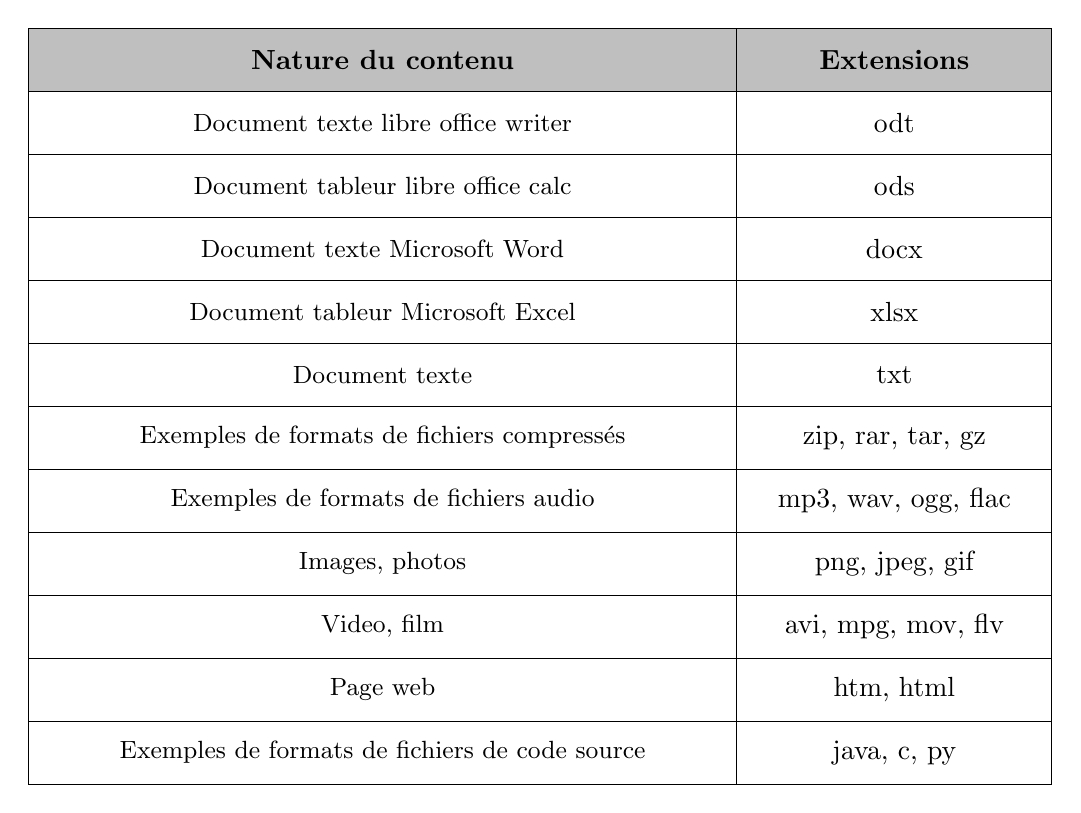
\begin{tikzpicture}
		\filldraw[fill=lightgray] (-1,8.8) rectangle (12,8);
		\draw (12,-.8) rectangle
		(-1,0) rectangle (12,0.8) rectangle (-1,1.6) 
		rectangle (12,2.4) rectangle (-1,3.2) 
		rectangle (12,4) rectangle (-1,4.8)
		rectangle (12,5.6) rectangle (-1,6.4)
		rectangle (12,7.2) rectangle (-1,8);
		\draw (8,-0.8) -- (8,8.8);
		
		\draw (3.5,8.4) node {\bf Nature du contenu};
		\draw (10,8.4) node {\bf Extensions};
		
		\draw (3.5,7.6) node {\small Document texte libre office writer};
		\draw (10,7.6) node { odt};
		
		\draw (3.5,6.8) node {\small Document tableur libre office calc};
		\draw (10,6.8) node {ods};
		
		\draw (3.5,6) node {\small Document texte Microsoft Word};
		\draw (10,6) node {docx};
		
		\draw (3.5,5.2) node {\small Document tableur Microsoft Excel};
		\draw (10,5.2) node {xlsx};
		
		\draw (3.5,4.4) node {\small Document texte};
		\draw (10,4.4) node {txt};
		
		\draw (3.5,3.6) node {\small Exemples de formats de fichiers compressés};
		\draw (10,3.6) node {zip, rar, tar, gz};
		
		\draw (3.5,2.8) node {\small Exemples de formats de fichiers audio};
		\draw (10,2.8) node {mp3, wav, ogg, flac};
		
		\draw (3.5,2) node {\small Images, photos};
		\draw (10,2) node {png, jpeg, gif};
		
		\draw (3.5,1.2) node {\small Video, film};
		\draw (10,1.2) node {avi, mpg, mov, flv};
		
		\draw (3.5,0.4) node {\small Page web};
		\draw (10,0.4) node {htm, html};
		
		\draw (3.5,-0.4) node {\small Exemples de formats de fichiers de code source};
		\draw (10,-0.4) node {java, c, py};
		
	\end{tikzpicture}
\end{center}

\subsection{L'arborescence}
Usuellement, les fichiers sont regroupés en \textbf{répertoires} ou \textbf{dossiers}. Un répertoire est un conteneur, c'est-à-dire q'il sert simplement à contenir des fichiers ou d'autres répertoires. Les répertoires vont s'imbriquer les uns dans les autres de manière a former une arborescence.

Pour comprendre cette idée d'arborescence, prenons l'exemple de comment un élève pourrait organiser ses documents de cours. Premièrement tous les documents sont stockés dans un armoire, c'est le dossier \textit{\textbf{racine}}. Dans ce dossier racine, il y a un classeur par matière enseigné au collège, chaque classeur correspond à un dossier. Les documents de chacun des classeurs peuvent être regroupés par thème dans des pochettes. Par exemple, dans le classeur géographique, on retrouve une pochette (un dossier) Europe qui contient tous les documents (fichiers) qui traitent de l'Europe.

\begin{figure}[!h]
	\centering
	\subfloat[Analogie]{\includegraphics[width=0.4\textwidth]{Images/OS/organisationfichiers}}
	\hspace{1cm}
	\subfloat[Représentation synthétique ]{\includegraphics[trim=0 0 100 50, width=0.45\textwidth]{Images/OS/arborescence2}}
	\caption{L'arborescence de fichiers et dossiers.}
\end{figure}\label{CourbeRepr}
Pour résumer: 
\begin{enumerate}
	\item Un {\bf dossier} peut comporter d’autres dossiers et des fichiers.
	\item Un {\bf fichier} est un ensemble organisé d'informations, désigné par un nom précis, que le système d'exploitation d'un ordinateur manipule comme une simple entité, dans sa mémoire persistante.
\end{enumerate}
L’organisation arborescente des fichiers n’est pas le seul moyen de structurer l’information : elle est en concurrence avec d’autres méthodes, parmi lesquelles l’utilisation de liens hypertextes, notion qui n’a pas été inventée pour structurer l’information, mais pour simplifier le mécanisme de référence dans une page web.

\subsection{Le dossier utilisateur}
Les systèmes d'exploitation multi-utilisateurs (ce qui est les cas de Linux, Mac OS X ou Windows) mettent à disposition à chacun de leurs utilisateurs un espace de stockage personnalisé. Cet espace sert principalement à stocker les données propres à l'utilisateur (documents, photos, ...). Un utilisateur peut modifier à sa guise son espace mais ne peut pas, en général, accéder à l'espace d'un autre utilisateur. Il existe cependant la possibilité de \textbf{partager} des dossiers entres plusieurs utilisateurs.

En fonction du système d'exploitation, le chemin d'accès au dossier utilisateur varie. Par exemples, sous
\begin{itemize}
	\item \textbf{Linux}, chaque utilisateur possède un dossier personnalisé dans le répertoire \lstinline{/home};
	\item \textbf{Mac OS X}, chaque utilisateur possède un dossier personnalisé dans le répertoire \lstinline{/Users};
	\item \textbf{Windows 10}, chaque utilisateur possède un dossier personnalisé dans le répertoire \lstinline{C:\Users};
\end{itemize}
\begin{figure}[h!]
	\centering
	\includegraphics[trim=0 0 0 0,width=0.8\textwidth]{Images/OS/dossier_home.png}
	\caption{Localisation du dossier utilisateur sous Linux, Mac OSX et Windows NT (différent dans les dernières versions de Windows) }
\end{figure}
Dans le dossier utilisateur, on trouve, par défaut, des sous dossiers du type "Mes documents", *mes images", "Téléchargement", "Bureau",...

\subsection{L'arborescence sous Unix (Ubuntu, Android, iOS)}

\begin{mydefinition}
	Un chemin est une liste de répertoire à traverser pour atteindre un fichier ou répertoire donné.
\end{mydefinition}
Tout fichier est référencé par son chemin d’accès, c’est à dire la description du chemin qu’il faut parcourir dans l’arborescence à partir d’un certain répertoire pour atteindre le fichier en question. Le chemin est spécifié par les noms des répertoires séparés par le caractère « / » et suivi du nom du fichier. Lorsqu’on commence la description du chemin par la racine, on dit que le \textbf{chemin est absolu}.
\begin{figure}[h!]
	\centering
	\includegraphics[trim=0 0 0 0,width=0.8\textwidth]{Images/OS/Exemple_arbo_linux}
	\caption{Un arborescence de dossier similaire à l'exemple des classeurs à été crée dans le répertoire du dossier personnel de l'utilisateur "mathieu". Ici, nous visualisons le contenu du répertoire \lstinline{Histoire} qui contient un unique fichier de format PDF et son chemin (absolu) est \lstinline{/home/mathieu/Armoire_de_classeurs/Histoire/Fiche_Genève_1900.pdf}.}
	\label{ex_chemin}
\end{figure}

\begin{important}
	Au collège Sismondi, seuls les enseignant ont un compte utilisateur personnalisé. Tous les élèves se connectent avec le compte  \lstinline{eleve-sismondi}. Dans ce cas, le dossier personnalisé est (en général ?) effacé à chaque nouvelle connexion. Par conséquent, vous devez absolument sauvegarder votre travail, soit sur un clé USB, soit sur un dossier dans le google Drive (\url{eduge.ch}).
\end{important}	
\begin{eclairage}
	 Il est aussi possible de décrire un fichier relativement à la position d’un autre répertoire ; on parle alors de \textbf{chemin relatif}. Dans ce cas, une remontée dans la hiérarchie (accès au dossier parent) est symbolisés par deux points « .. ». Dans l'exemple de la figure \ref{ex_chemin}, le chemin qui part du dossier courant \lstinline{Histoire} vers le dossier \lstinline{Pochette_Europe} est \lstinline{../Géographie/Pochette_Europe}.
\end{eclairage}

Il existe deux moyens pour naviguer dans l'arborescence de fichiers:
\begin{itemize}
	\item Des commandes \lstinline{shell} qui s'utilisent avec une interface en lignes de commandes.
	\item Un explorateur de fichier qui est un programme avec une interface graphique utilisateur.
\end{itemize}

\subsubsection{Navigation avec des lignes de commande*}
Il est possible d’explorer cette arborescente en utilisant un terminal (ou le powershell) et les quelques instructions suivantes
\begin{itemize}
	\item \lstinline{pwd} affiche le répertoire courant ;
	\item \lstinline{ls} affiche le contenu du répertoire courant ;
	\item \lstinline{cd} change le répertoire courant ;
	\item \lstinline{mv} déplace (et renomme) un fichier ou un dossier ;
	\item \lstinline{cp} copie (et renomme) un fichier ;
	\item \lstinline{rm} supprime un fichier ;
	\item \lstinline{mkdir} crée un nouveau répertoire (vide) ;
	\item \lstinline{rmdir} supprime un répertoire vide.
\end{itemize}

 Initialement, le répertoire courant est le dossier personnel de l'utilisateur. Vous pouvez vérifier cette information avec la commande \lstinline{pwd}.
\begin{figure}[h!]
	\centering
	\includegraphics[trim=0 0 0 0,width=0.8\textwidth]{Images/OS/navigation_terminal}
	\caption{L'explorateur de fichiers à partir de lignes de commandes.}
\end{figure}
\begin{important}
	Lorsque l'on supprime un fichier ou un dossier avec les commandes \lstinline{rm} et \lstinline{rmdir}, il sera définitivement supprimé! Il n'ira pas dans la corbeille.
\end{important}	

\subsubsection{Explorateur de fichier}
L'explorateur de fichier permet de naviguer dans les répertoires au moyen de la souris. En général, on trouve un panneau sur la gauche avec un accès rapide au dossier les plus utilisés. Le contenu d'un dossier s'affiche lorsque l'on clique dessus. 
\begin{figure}[h!]
	\centering
	\includegraphics[trim=0 0 0 0,width=0.6\textwidth]{Images/OS/dolphin}
	\caption{Accès aux répertoires fichier depuis un terminal.}
\end{figure}
